\begin{figure}[!ht]
	\centering
	\addtolength{\tabcolsep}{-3pt}
	\begin{tabular}{cccc}
		\raisebox{27pt}{
\includegraphics[width=0.25\columnwidth]{bayesian/fig11/target.jpg}} &
		\raisebox{0pt}{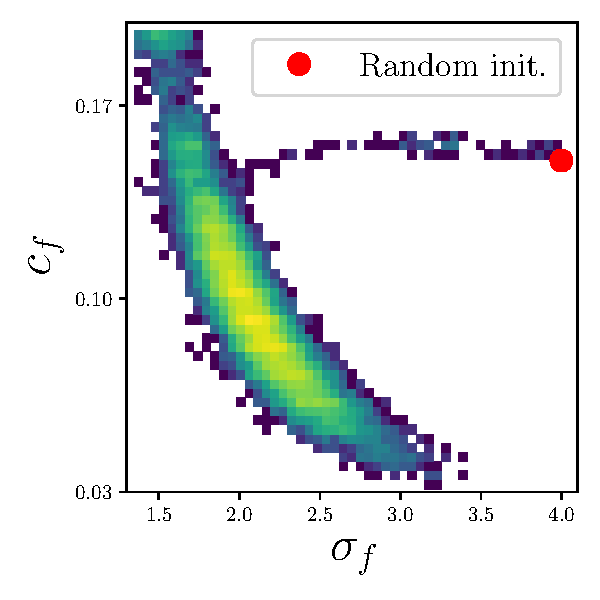
\includegraphics[width=0.32\columnwidth]{bayesian/fig11/sample1.pdf}} &
		\raisebox{0pt}{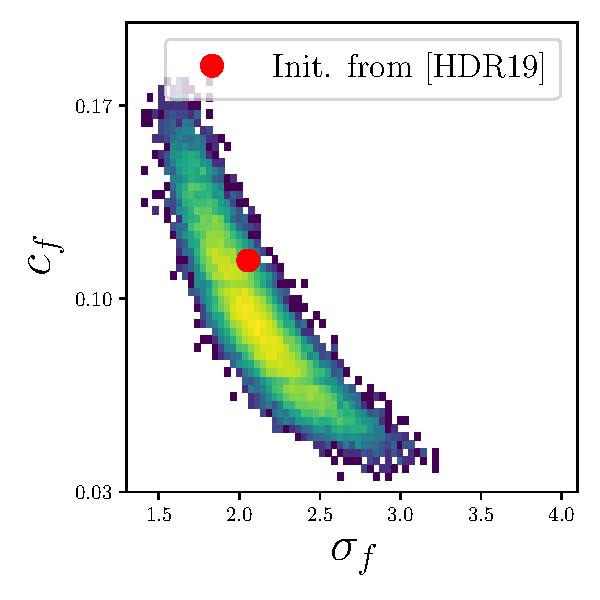
\includegraphics[width=0.32\columnwidth]{bayesian/fig11/sample2.pdf}} &
		\raisebox{50pt}{\rotatebox{90}{$N=22500$}} \\[-1.2em]
		Target & (a) & (b)
	\end{tabular}
	\caption[Initialization]{\label{fig:bayesian:hu2}
		\textbf{Initialization} of our sampling with the method of Hu et al. \cite{hu2019novel} on a synthetic bumpy surface example. The figure shows joint posterior distributions over two parameters using different initializations: a random initialization drawn from the prior (a) and the prediction of [HDR19] (b). As we can see, starting from the result of [HDR19] can shorten the burn-in phase of the MCMC sampling process.
	}
\end{figure}
